% !TeX root = ../index.tex
\chapter{Web Service Proposal}
% 10 marks
\section{Project Name}

Hibari API

\section{Overview of the Project}

The project will provide extra statistics related to users and media on Kitsu, which would require hundreds of requests to generate client-side. The provided statistics from this project can then be used to provide users insights into what they are watching/reading and how they compare to other users on the service.

\section{External Web Services to Be Consumed}

The Web Service I will be consuming in this project is Kitsu\footnote{\url{https://kitsu.io}}, an anime \& manga discovery and tracking service (similar to IMDb). Its Web Service published as a RESTful API\footnote{\url{https://kitsu.docs.apiary.io}} that uses the JSON:API\footnote{\url{http://jsonapi.org}} specification.

From Kitsu's API I will be storing user IDs, user's library entries (completion status, rating and progress) and anime data (airing status, start date and episode count).

\newpage
\section{What Will Be Exposed in My Web Service}
\fxwarning{In progress}

% \textbf{Note:} \textit{media} refers to \textit{anime} and \textit{manga} exposed as separate API methods that share the same functionality and output.

\begin{enumerate}
  \item\label{computed-stats} Computed statistics of media ratings%\fxnote{Maybe also Chebyshev's Theorem and Coefficient of Variation}
    \begin{enumerate}
      \item Count
      \item Mean
      \item Median
      \item Mode
      \item Variance
      \item Standard deviation
      \item Raw rating frequency - key-value pair of \texttt{\{ rating: occurance \}}
    \end{enumerate}
  \item User libraries
    \begin{enumerate}
      \item Statistics of media in the user's library (see \ref{computed-stats}.)
      \item Statistics of media in the user's library grouped by airing year (see \ref{computed-stats}.)
      \item Statistics of media in the user's library grouped by category (see \ref{computed-stats}.)
      \item Total episodes/chapters seen
      \item Total episodes/chapters seen per status type (Currently Watching, Plan to Watch, Completed, On Hold and Dropped)
      \item Total episodes/chapters not seen
      \item Total episodes/chapters not seen per status type
    \end{enumerate}
  \item Categories
    \begin{enumerate}
      \item Statistics of media in a category (see \ref{computed-stats})
      \item Statistics of media in a category grouped by airing year (see \ref{computed-stats}.)
    \end{enumerate}
  \item Media
    \begin{enumerate}
      \item Rank in category (position and percentile)
    \end{enumerate}
\end{enumerate}

\newpage
\section{Initial Database Schema}

\begin{figure}[H]
  \caption{Schema}
  \centering
  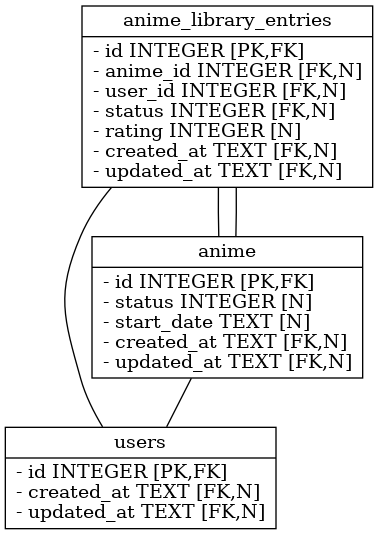
\includegraphics[width=.5\textwidth]{1-schema}
\end{figure}

\newpage
\section{Initial Wireframes / UI Ideas}
\fxerror{Not started}
